\documentclass[11pt,a4paper]{article}

% ============================================================================
% PACKAGES
% ============================================================================
\usepackage[utf8]{inputenc}
\usepackage[T1]{fontenc}
\usepackage{amsmath,amssymb,amsthm,amsfonts,mathrsfs}
\usepackage{mathtools}
\usepackage{geometry}
\usepackage{fancyhdr}
\usepackage{everypage}
\usepackage{tikz}
\usepackage{tikz-cd}
\usepackage{hyperref}
\usepackage{cleveref}
\usepackage{enumitem}
\usepackage{listings}
\usepackage{xcolor}
\usepackage{abstract}
\usepackage{titlesec}
\usepackage{booktabs}
\usepackage{caption}
\usepackage{float}
\usepackage{stmaryrd}
\usepackage{setspace}
\usepackage{graphicx}

\geometry{margin=1in, left=1.35in}
\onehalfspacing

% ============================================================================
% GROKRXIV DOI SIDEBAR
% ============================================================================
\definecolor{grokgray}{RGB}{110,110,110}
\AddEverypageHook{%
  \ifnum\value{page}=1
    \begin{tikzpicture}[remember picture, overlay]
      \node[
        rotate=90,
        anchor=south,
        font=\Large\sffamily\bfseries\color{grokgray},
        inner sep=0pt
      ] at ([xshift=38pt, yshift=0.52\paperheight]current page.south west)
      {GrokRxiv:2026.04.hott-hallucination-synthesis\quad
       [\,cs.AI / math.AT\,]\quad
       14 Apr 2026};
    \end{tikzpicture}
  \fi
}

% ============================================================================
% THEOREM ENVIRONMENTS
% ============================================================================
\theoremstyle{plain}
\newtheorem{theorem}{Theorem}[section]
\newtheorem{lemma}[theorem]{Lemma}
\newtheorem{proposition}[theorem]{Proposition}
\newtheorem{corollary}[theorem]{Corollary}
\newtheorem{conjecture}[theorem]{Conjecture}
\theoremstyle{definition}
\newtheorem{definition}[theorem]{Definition}
\newtheorem{example}[theorem]{Example}
\newtheorem{construction}[theorem]{Construction}
\newtheorem{axiom}[theorem]{Axiom}
\theoremstyle{remark}
\newtheorem{remark}[theorem]{Remark}
\newtheorem{notation}[theorem]{Notation}

% ============================================================================
% CODE LISTINGS
% ============================================================================
\definecolor{codebg}{HTML}{F7F7F7}
\definecolor{codegreen}{HTML}{228B22}
\definecolor{codepurple}{HTML}{7B2D8B}
\definecolor{codeorange}{HTML}{D35400}

\lstdefinestyle{haskellstyle}{
  language=Haskell,
  basicstyle=\ttfamily\small,
  backgroundcolor=\color{codebg},
  keywordstyle=\color{codepurple}\bfseries,
  commentstyle=\color{codegreen}\itshape,
  stringstyle=\color{codeorange},
  breaklines=true,
  frame=single,
  rulecolor=\color{grokgray!40},
  numbers=left,
  numberstyle=\tiny\color{grokgray},
  numbersep=5pt,
  xleftmargin=14pt,
  framexleftmargin=12pt,
  columns=flexible,
  morekeywords={where,data,type,class,instance,deriving,newtype,family,
    forall,GADT,DataKinds,TypeFamilies,PolyKinds,RankNTypes,
    Maybe,Just,Nothing,Either,Left,Right,Bool,True,False,
    SemType,SemTerm,Context,PathEvidence,Derivation,Chain,
    TopologicalObstruction,HallucinationType,HomologyClass,
    GroundingResult,Simplex,KnowledgeComplex,Fiber,HoTTLM,
    PersistenceBar,FundGroupoid,VietorisRips,SemanticMonad,
    DetectionResult,GenerationResult,SynthesisEngine},
  literate={->}{{$\to$}}2 {=>}{{$\Rightarrow$}}2 {<-}{{$\leftarrow$}}2
           {::}{{$\dblcolon$}}2
}
\lstset{style=haskellstyle}

% ============================================================================
% MACROS
% ============================================================================
\newcommand{\CC}{\mathbf{C}}
\newcommand{\Sem}{\mathbf{Sem}}
\newcommand{\Lang}{\mathbf{Lang}}
\newcommand{\Vect}{\mathbf{Vect}}
\newcommand{\Grpd}{\boldsymbol{\infty}\text{-}\mathbf{Grpd}}
\newcommand{\Set}{\mathbf{Set}}
\newcommand{\Type}{\mathsf{Type}}
\newcommand{\Prop}{\mathsf{Prop}}
\newcommand{\refl}{\mathsf{refl}}
\newcommand{\transport}{\mathsf{transport}}
\newcommand{\ua}{\mathsf{ua}}
\newcommand{\id}{\mathrm{id}}
\newcommand{\Hom}{\mathrm{Hom}}
\newcommand{\VR}{\mathrm{VR}}
\newcommand{\im}{\mathrm{im}}
\newcommand{\ob}{\mathrm{ob}}
\newcommand{\op}{\mathrm{op}}
\newcommand{\Nat}{\mathrm{Nat}}
\newcommand{\PSh}{\mathrm{PSh}}
\newcommand{\vocab}{\mathcal{V}}
\newcommand{\Hall}{\mathsf{Hall}}
\newcommand{\hTop}{\mathsf{hTop}_*}
\newcommand{\Detect}{\mathsf{Detect}}
\newcommand{\Generate}{\mathsf{Generate}}
\newcommand{\SemanticT}{\mathsf{T}}
\DeclareMathOperator{\coker}{coker}
\DeclareMathOperator{\Fib}{Fib}
\DeclareMathOperator{\holim}{holim}
\DeclareMathOperator{\hocolim}{hocolim}
\DeclareMathOperator{\Map}{Map}
\DeclareMathOperator{\Aut}{Aut}
\DeclareMathOperator{\Hol}{Hol}

\hypersetup{
  colorlinks=true,
  linkcolor=blue!70!black,
  citecolor=blue!70!black,
  urlcolor=blue!70!black
}

% ============================================================================
% TITLE
% ============================================================================
\title{%
  \textbf{The HoTT Hallucination Framework}\\[6pt]
  \large A Unified Theory of Semantic Correctness for Language Models\\
  via Homotopy Type Theory%
}

\author{%
  Matthew Long\thanks{%
    Corresponding author. \texttt{matthew@yonedaai.com} \;\textbullet\; \url{https://yonedaai.com}%
  }\\[2pt]
  \textit{YonedaAI Research Collective}\\
  \textit{Magneton Labs LLC}\\
  Chicago, IL, USA
}

\date{April 2026}

% ============================================================================
% DOCUMENT
% ============================================================================
\begin{document}
\maketitle
\thispagestyle{empty}

% ============================================================================
% ABSTRACT
% ============================================================================
\begin{abstract}
\noindent
We present a unified framework for semantic correctness in large language models (LLMs) that synthesizes two complementary research threads: \emph{topological detection} of hallucination via homotopy groups and homology, and \emph{type-theoretic generation} via certified inhabitation search in Homotopy Type Theory (HoTT). Our central construction is the \textbf{detection-generation duality}: detection is the problem of checking whether a global section of a semantic sheaf exists, while generation is the problem of constructing such a section. We prove these operations form an adjoint pair $\Generate \dashv \Detect$ on the semantic category $\Sem$, and that the composite $\SemanticT = \Detect \circ \Generate$ is a monad on $\Sem$---the \textbf{semantic monad}---whose unit maps semantic types to their verified versions and whose multiplication collapses redundant verification. We formalize the ambient mathematical universe as an $\infty$-topos of semantic types, where objects are homotopy types, morphisms are certified derivations, and the internal logic is HoTT itself. Within this framework, we prove the \textbf{Completeness Theorem}: the Hallucination--Homotopy Correspondence (HHC) together with type-theoretic generation yields a \emph{complete} system in which every hallucination is detected and generation never produces undetected hallucinations. We provide a concrete proof-of-concept architecture wrapping an LLM with a type-checking layer implementing a generate-check-abstain loop, with persistent homology for real-time topological monitoring. The framework is formalized in Haskell.

\medskip
\noindent\textbf{Keywords:} Homotopy Type Theory, $\infty$-Topos, Adjoint Functors, Monads, Sheaf Cohomology, LLM Hallucination, Persistent Homology, Algebraic Topology, Categorical Semantics, Type Inhabitation
\end{abstract}

\tableofcontents
\newpage

% ============================================================================
% 1. INTRODUCTION
% ============================================================================
\section{Introduction}\label{sec:intro}

The hallucination problem in large language models---the generation of fluent, confident text that is factually incorrect or entirely fabricated---has resisted every attempted remedy. Scaling laws \cite{openai2023gpt4}, reinforcement learning from human feedback \cite{ouyang2022training}, retrieval-augmented generation \cite{lewis2020retrieval}, chain-of-thought prompting, constitutional AI, and self-consistency decoding have all failed to eliminate hallucination. We have argued in prior work \cite{long2026homotopical,long2026hhc} that this resistance is not accidental but structural: hallucination is a \emph{theorem}, not a bug.

This paper is the capstone synthesis. It unifies two complementary threads developed in our preceding papers:

\begin{enumerate}[leftmargin=*]
\item \textbf{Thread 1 --- Topological Detection} \cite{long2026hhc}. Five hallucination types are classified via the Hallucination--Homotopy Correspondence (HHC): circular reasoning ($\pi_1$), unjustified inference ($\pi_0$), inconsistent justifications ($\pi_2$), fabricated entity chains ($H_n$), and compositional drift (holonomy). Detection reduces to computing homotopy-theoretic invariants of a simplicial knowledge complex $\mathcal{K}_\bullet$.

\item \textbf{Thread 2 --- Type-Theoretic Generation} \cite{long2026homotopical}. Five generation principles replace statistical next-token prediction: generation as type inhabitation search, certified derivations, abstention on empty types, context as fibration, and attention as weighted limit.
\end{enumerate}

The key insight of the present work is that \emph{detection and generation are not independent operations}. They stand in a precise categorical relationship: detection is section-existence checking on a semantic sheaf, generation is section construction, and they form an \textbf{adjoint pair}. The composite $\SemanticT = \Generate \circ \Detect$ inherits monad structure. The ambient mathematical universe is an $\infty$-topos whose internal logic is HoTT itself. Within this framework, we prove that the combined system is \emph{complete}: every hallucination is detected, and generation never produces undetected hallucinations.

\subsection{Contributions}

This synthesis paper makes the following contributions:

\begin{enumerate}[leftmargin=*,nosep]
  \item We establish the \textbf{Detection-Generation Duality} (\Cref{sec:duality}): detection and generation form an adjoint pair $\Generate \dashv \Detect$ on $\Sem$.
  \item We construct the \textbf{Semantic Monad} $\SemanticT = \Generate \circ \Detect$ (\Cref{sec:monad}) and prove it satisfies the monad laws with semantic interpretations.
  \item We formalize the ambient framework as an \textbf{$\infty$-Topos of Semantic Types} (\Cref{sec:topos}) where the internal logic is HoTT.
  \item We develop the \textbf{Sheaf-Theoretic Formulation} (\Cref{sec:sheaf}) unifying obstruction-theoretic detection with section-constructive generation.
  \item We prove the \textbf{Completeness Theorem} (\Cref{sec:completeness}): HHC + type-theoretic generation = a complete hallucination-free system.
  \item We provide a concrete \textbf{POC Architecture} (\Cref{sec:architecture}) with tikz diagrams and a full \textbf{Haskell formalization} (\Cref{sec:haskell}).
  \item We design an \textbf{Experimental Framework} (\Cref{sec:experiments}) for empirical validation.
\end{enumerate}

\subsection{Related Work}

The categorical and topological approach to language model semantics builds on several research traditions.

\paragraph{Categorical Semantics of Language.} The DisCoCat framework of Coecke, Sadrzadeh, and Clark \cite{coecke2010mathematical} models meaning compositionally via functors from grammar categories to vector spaces. Our framework replaces the codomain $\Vect$ with $\Grpd$, preserving higher-dimensional structure.

\paragraph{Homotopy Type Theory.} The HoTT Book \cite{hottbook} provides the foundational framework. Voevodsky's univalence axiom \cite{voevodsky2010univalent} is central to our semantic equivalence constraints. Cubical type theory \cite{cohen2018cubical} provides computational content.

\paragraph{Topological Data Analysis.} Carlsson's foundational work \cite{carlsson2009topology} and the persistent homology of Edelsbrunner and Harer \cite{edelsbrunner2010computational} underpin our practical detection algorithms. Naitzat, Zhitnikov, and Lim \cite{naitzat2020topology} study the topology of neural network activations.

\paragraph{Hallucination in LLMs.} The survey of Ji et al.\ \cite{ji2023survey} taxonomizes hallucination types. Huang et al.\ \cite{huang2023survey} survey detection methods. Li \cite{li2025} studies inference-time interventions. None of these works provide a structural mathematical explanation for \emph{why} hallucination occurs.

\paragraph{Topos Theory and Logic.} Mac Lane and Moerdijk \cite{maclane1994sheaves} provide the topos-theoretic foundations. Johnstone \cite{johnstone2002sketches} develops the connection between topoi and logic that we exploit for the internal language interpretation.

\subsection{Paper Outline}

\Cref{sec:review} reviews the two preceding papers. \Cref{sec:duality} establishes the detection-generation duality. \Cref{sec:monad} constructs the semantic monad. \Cref{sec:topos} develops the $\infty$-topos framework. \Cref{sec:sheaf} gives the sheaf-theoretic formulation. \Cref{sec:completeness} proves the completeness theorem. \Cref{sec:architecture} presents the POC architecture. \Cref{sec:haskell} gives the Haskell formalization. \Cref{sec:experiments} outlines the experimental design. \Cref{sec:discussion} discusses implications. \Cref{sec:conclusion} concludes.


% ============================================================================
% 2. REVIEW OF THE TWO THREADS
% ============================================================================
\section{Review of the Two Threads}\label{sec:review}

We briefly recapitulate the essential constructions from our two preceding papers, establishing notation for the synthesis.

\subsection{Thread 1: Topological Detection}\label{sec:review-detection}

The first paper \cite{long2026hhc} establishes the Hallucination--Homotopy Correspondence (HHC). The key constructions are:

\begin{definition}[Semantic $\infty$-Groupoid]\label{def:semtype-review}
Semantic meaning is modeled as a homotopy type $A : \Type$ whose cells encode:
\begin{itemize}[nosep]
  \item \textbf{0-cells} (points $a : A$): valid propositions or claims of type $A$.
  \item \textbf{1-cells} (paths $p : a =_A b$): justifications or entailments between claims.
  \item \textbf{2-cells} ($\alpha : p =_{a =_A b} q$): equivalences between justifications.
  \item \textbf{$n$-cells}: higher coherence data.
\end{itemize}
\end{definition}

\begin{definition}[Knowledge Complex $\mathcal{K}_\bullet$]\label{def:knowledge-complex-review}
Given a knowledge base $\mathcal{K}$, the knowledge simplicial complex $\mathcal{K}_\bullet$ has:
\begin{itemize}[nosep]
  \item $\mathcal{K}_0$: grounded atomic facts (0-simplices).
  \item $\mathcal{K}_1$: pairs of mutually consistent facts connected by justification (1-simplices).
  \item $\mathcal{K}_n$: $(n{+}1)$-tuples with $n$-dimensional justificatory structure.
\end{itemize}
The associated chain complex $C_n(\mathcal{K}_\bullet) \xrightarrow{\partial_n} C_{n-1}(\mathcal{K}_\bullet)$ satisfies $\partial_n \circ \partial_{n+1} = 0$.
\end{definition}

\begin{theorem}[Hallucination--Homology Correspondence {\cite[Theorem~3.1]{long2026hhc}}]\label{thm:hhc-review}
A chain $\sigma \in C_n(\mathcal{K}_\bullet)$ of claims generated by a language model is hallucinated if and only if $[\sigma] \neq 0 \in H_n(\mathcal{K}_\bullet; \mathbb{Z})$.
\end{theorem}

\begin{theorem}[HHC Classification {\cite[Theorem~4.1]{long2026hhc}}]\label{thm:hhc-classification-review}
The complete classification of hallucination types by homotopy-theoretic invariants is:
\begin{center}
\begin{tabular}{llll}
\toprule
\textbf{Hallucination Type} & \textbf{Invariant} & \textbf{Obstruction} \\
\midrule
Unjustified inference & $\pi_0$ & Disconnection \\
Circular reasoning & $\pi_1 \neq 0$ & Non-contractible loop \\
Inconsistent justifications & $\pi_2 \neq 0$ & Incoherent 2-cell \\
Fabricated entity chain & $H_n \neq 0$ & Homological hole \\
Compositional drift & $\Hol \neq \id$ & Transport anomaly \\
\bottomrule
\end{tabular}
\end{center}
\end{theorem}

\begin{theorem}[Fundamental Obstruction {\cite[Theorem~5.1]{long2026hhc}}]\label{thm:obstruction-review}
Let $\Sem$ be a semantic category with $\pi_k(\Sem) \neq 0$ for some $k \geq 1$. Then there exists no faithful functor $F\colon \Sem \to \CC$ where $\CC$ is contractible.
\end{theorem}

\subsection{Thread 2: Type-Theoretic Generation}\label{sec:review-generation}

The second paper \cite{long2026homotopical} develops the HoTT-LM architecture based on five generation principles:

\begin{enumerate}[leftmargin=*,nosep]
\item \textbf{Generation as Type Inhabitation}: Replace $\arg\max_t P(t \mid \text{ctx})$ with: find $a$ such that $\Gamma \vdash a : A$ has derivation $\delta$.
\item \textbf{Certified Derivations}: Every generated term $a : A$ comes with a derivation tree $\delta$ witnessing $\Gamma \vdash a : A$.
\item \textbf{Abstention on Empty Types}: When $A$ is uninhabited, return $\bot$ rather than hallucinate.
\item \textbf{Context as Fibration}: The context window is a dependent telescope, not a flat token sequence.
\item \textbf{Attention as Limit}: Attention computes a weighted limit in $\Sem$, not a weighted sum in $\Vect$.
\end{enumerate}

\begin{definition}[HoTT-LM]\label{def:hottlm-review}
A Homotopy Type-Theoretic Language Model is a quadruple $(\mathsf{generate}, \mathsf{verify}, \mathsf{transport}, \mathsf{unify})$ where:
\begin{align}
\mathsf{generate} &: \Gamma \times A \to \mathsf{Maybe}(a, \delta) \\
\mathsf{verify} &: \Gamma \times a \times A \to \mathsf{Maybe}(\delta) \\
\mathsf{transport} &: \Gamma \times a \times p \to \mathsf{Maybe}(a') \\
\mathsf{unify} &: a \times b \to \mathsf{Maybe}(p)
\end{align}
with $a : A$, $\delta$ a derivation, $p$ a path evidence, and $\mathsf{Maybe}$ encoding possible abstention.
\end{definition}

\subsection{The Gap: What Neither Thread Provides Alone}

Thread 1 tells us \emph{how to detect} hallucination but not \emph{how to generate} correct output. Thread 2 tells us \emph{how to generate} but assumes the type-theoretic infrastructure is already in place and does not address the topological structure of the failure modes it avoids. Neither thread addresses:
\begin{itemize}[nosep]
  \item The categorical relationship between detection and generation.
  \item Whether the combined system is \emph{complete} (all hallucinations caught, all correct claims producible).
  \item The ambient mathematical universe in which both threads operate.
  \item A concrete architecture implementing both simultaneously.
\end{itemize}

The synthesis that follows closes each of these gaps.


% ============================================================================
% 3. THE DETECTION-GENERATION DUALITY
% ============================================================================
\section{The Detection-Generation Duality}\label{sec:duality}

We now establish the central structural insight of this paper: detection and generation, far from being independent operations, are adjoint functors on the semantic category.

\subsection{The Semantic Category Revisited}

\begin{definition}[Semantic Category $\Sem$]\label{def:sem-cat}
The semantic category $\Sem$ has:
\begin{itemize}[nosep]
  \item \textbf{Objects}: Semantic types $A : \Type$ (homotopy types in the sense of \Cref{def:semtype-review}).
  \item \textbf{Morphisms}: Certified derivations $\delta : \Gamma \vdash a : A$, i.e., terms together with their typing judgments.
  \item \textbf{Composition}: Transitivity of entailment: if $\Gamma \vdash f : A \to B$ and $\Gamma \vdash g : B \to C$, then $\Gamma \vdash g \circ f : A \to C$.
  \item \textbf{Identity}: Reflexivity of meaning: $\id_A = \refl_A$.
\end{itemize}
\end{definition}

\begin{definition}[Category of Claims $\mathsf{Claim}$]\label{def:claim-cat}
The category $\mathsf{Claim}$ has:
\begin{itemize}[nosep]
  \item \textbf{Objects}: Raw claims $\hat{a}$ (strings generated by an LLM, prior to verification).
  \item \textbf{Morphisms}: Textual transformations (paraphrase, elaboration, summarization).
  \item \textbf{No path structure}: $\mathsf{Claim}$ is a discrete category enriched only over $\Set$.
\end{itemize}
\end{definition}

\begin{definition}[Category of Verified Claims $\mathsf{VClaim}$]\label{def:vclaim-cat}
The category $\mathsf{VClaim}$ is the full subcategory of $\Sem$ consisting of types $A$ for which there exists a grounded term $a : A$ with a complete derivation $\delta$. It is the ``image'' of successful generation.
\end{definition}

\subsection{Detection as a Functor}

\begin{definition}[Detection Functor]\label{def:detect-functor}
The \textbf{detection functor} $\Detect\colon \mathsf{Claim} \to \Sem$ maps:
\begin{itemize}[nosep]
  \item A raw claim $\hat{a}$ to its semantic type $A_{\hat{a}} : \Type$---the ``what is being claimed.''
  \item A textual transformation $f\colon \hat{a} \to \hat{b}$ to the induced morphism $\Detect(f)\colon A_{\hat{a}} \to A_{\hat{b}}$ in $\Sem$.
\end{itemize}
The functor $\Detect$ computes the \emph{semantic structure} of a claim: its type, its required path evidence, and the topological obstructions (if any) preventing it from being grounded. Concretely, $\Detect$ performs:
\begin{enumerate}[nosep]
  \item \textbf{Type assignment}: Parse claim $\hat{a}$ to determine its semantic type $A$.
  \item \textbf{Context extraction}: Determine the context $\Gamma$ in which $\hat{a}$ is asserted.
  \item \textbf{Obstruction computation}: Compute $[\sigma] \in H_n(\mathcal{K}_\bullet)$ and $\pi_k$ invariants.
  \item \textbf{Verdict}: Return $(\Gamma, A, \text{obstructions})$.
\end{enumerate}
\end{definition}

\begin{remark}\label{rem:detect-enrichment}
The detection functor is enriched over the poset of obstruction classes: for each claim, it produces not just a binary ``hallucinated or not'' but a \emph{graded} assessment indexed by homotopy and homology groups. This enrichment is essential for the adjunction.
\end{remark}

\subsection{Generation as a Functor}

\begin{definition}[Generation Functor]\label{def:generate-functor}
The \textbf{generation functor} $\Generate\colon \Sem \to \mathsf{Claim}$ maps:
\begin{itemize}[nosep]
  \item A semantic type $A$ in context $\Gamma$ to a generated claim $\hat{a}$ (or $\bot$ if $A$ is uninhabited).
  \item A morphism $\delta : A \to B$ in $\Sem$ to the corresponding textual transformation.
\end{itemize}
Generation is type inhabitation search: given $\Gamma$ and $A$, find $a$ such that $\Gamma \vdash a : A$.
\end{definition}

\subsection{The Adjunction}

\begin{theorem}[Detection-Generation Adjunction]\label{thm:adjunction}
There is an adjunction:
\[
\Generate \dashv \Detect \colon \Sem \to \mathsf{Claim}
\]
That is, for every raw claim $\hat{a} \in \mathsf{Claim}$ and semantic type $A \in \Sem$:
\[
\Hom_{\mathsf{Claim}}(\Generate(A), \hat{a}) \cong \Hom_{\Sem}(A, \Detect(\hat{a}))
\]
naturally in $A$ and $\hat{a}$.
\end{theorem}

\begin{proof}
We construct the adjunction by exhibiting the unit and counit.

\emph{Unit} $\eta\colon \id_{\Sem} \Rightarrow \Detect \circ \Generate$. For a semantic type $A$, the unit $\eta_A\colon A \to \Detect(\Generate(A))$ maps $A$ to the semantic type assigned by detection to the claim generated from $A$. Since generation produces a term of type $A$ (when $A$ is inhabited), detection recovers $A$; the unit is the canonical map witnessing this.

\emph{Counit} $\varepsilon\colon \Generate \circ \Detect \Rightarrow \id_{\mathsf{Claim}}$. For a raw claim $\hat{a}$, the counit $\varepsilon_{\hat{a}}\colon \Generate(\Detect(\hat{a})) \to \hat{a}$ maps the re-generated version of $\hat{a}$ (after detection and re-generation) back to $\hat{a}$. This is the ``verification map'': it witnesses that re-generating from the detected semantic type produces a claim equivalent to the original (when the original is non-hallucinated).

\emph{Triangle identities}. We must verify:
\begin{enumerate}[nosep]
  \item $\varepsilon_{\Generate(A)} \circ \Generate(\eta_A) = \id_{\Generate(A)}$: generating from $A$, detecting the result, re-generating, and then applying the counit recovers the original generation. This holds because generation from a fully-specified type is deterministic (up to the choice of inhabitant).
  \item $\Detect(\varepsilon_{\hat{a}}) \circ \eta_{\Detect(\hat{a})} = \id_{\Detect(\hat{a})}$: detecting $\hat{a}$, generating from the detected type, re-detecting, and applying the unit recovers the original detection. This holds because detection is idempotent on well-typed claims.
\end{enumerate}
\end{proof}

\begin{remark}[Semantic Content of the Adjunction]\label{rem:adjunction-meaning}
The adjunction $\Generate \dashv \Detect$ encodes the following duality:
\begin{itemize}[nosep]
  \item $\Generate$ is the \emph{free} construction: given a semantic specification, produce the ``most natural'' claim satisfying it.
  \item $\Detect$ is the \emph{forgetful} construction: given a raw claim, extract its underlying semantic structure.
  \item The adjunction says that the ``best'' way to produce a claim of type $A$ (generation) is determined by the ``best'' way to detect type $A$ in claims (detection), and vice versa.
\end{itemize}
This is analogous to the free-forgetful adjunction $F \dashv U\colon \mathsf{Grp} \to \Set$, where the group generated by a set $S$ is determined by the elements of any group $G$ that $S$ maps into.
\end{remark}

\begin{corollary}[Hallucination as Adjunction Failure]\label{cor:hall-adjunction}
A claim $\hat{a}$ is hallucinated if and only if the counit $\varepsilon_{\hat{a}}$ is not an isomorphism: the re-generated version $\Generate(\Detect(\hat{a}))$ differs from $\hat{a}$ because detection reveals obstructions that generation cannot overcome.
\end{corollary}

The adjunction is summarized by the following commutative diagram:

\begin{center}
\begin{tikzcd}[column sep=large, row sep=large]
\Sem \arrow[r, bend left=25, "\Generate"{name=F}] \arrow[r, phantom, "\bot"] & \mathsf{Claim} \arrow[l, bend left=25, "\Detect"{name=U}]
\arrow[from=F, to=U, phantom, "\dashv"]
\end{tikzcd}
\end{center}


% ============================================================================
% 4. THE SEMANTIC MONAD
% ============================================================================
\section{The Semantic Monad}\label{sec:monad}

Every adjunction gives rise to a monad. The adjunction $\Generate \dashv \Detect$ produces the \textbf{semantic monad} $\SemanticT$ on $\Sem$.

\subsection{Construction}

\begin{definition}[Semantic Monad]\label{def:semantic-monad}
The \textbf{semantic monad} is the endofunctor $\SemanticT = \Detect \circ \Generate\colon \Sem \to \Sem$ equipped with:
\begin{itemize}[nosep]
  \item \textbf{Unit} $\eta\colon \id_{\Sem} \Rightarrow \SemanticT$: maps a semantic type $A$ to the semantics of its generated realization. This is the ``claim a type and generate evidence'' operation.
  \item \textbf{Multiplication} $\mu\colon \SemanticT^2 \Rightarrow \SemanticT$: collapses double verification. $\mu_A\colon \Detect(\Generate(\Detect(\Generate(A)))) \to \Detect(\Generate(A))$ says that verifying a verified claim adds nothing.
\end{itemize}
\end{definition}

\begin{theorem}[Monad Laws]\label{thm:monad-laws}
$(\SemanticT, \eta, \mu)$ satisfies the monad laws:
\begin{enumerate}[nosep]
  \item \textbf{Left unit}: $\mu \circ \eta_{\SemanticT} = \id_{\SemanticT}$.
  \item \textbf{Right unit}: $\mu \circ \SemanticT(\eta) = \id_{\SemanticT}$.
  \item \textbf{Associativity}: $\mu \circ \mu_{\SemanticT} = \mu \circ \SemanticT(\mu)\colon \SemanticT^3 \Rightarrow \SemanticT$.
\end{enumerate}
\end{theorem}

\begin{proof}
These follow formally from the triangle identities of the adjunction $\Generate \dashv \Detect$ (\Cref{thm:adjunction}). Explicitly:

\emph{Left unit.} $\mu_A \circ \eta_{\SemanticT(A)} = \mu_A \circ \eta_{\Detect(\Generate(A))}$. The unit $\eta$ takes the already-verified type $\Detect(\Generate(A))$ and re-generates and re-detects it. The multiplication $\mu$ then collapses the double verification. By the triangle identity (1) of the adjunction, this composite is the identity.

\emph{Right unit.} $\mu_A \circ \SemanticT(\eta_A) = \mu_A \circ \Detect(\Generate(\eta_A))$. Here $\eta_A$ is applied inside, and then the outer verification collapses. By triangle identity (2), this is the identity.

\emph{Associativity.} For $\SemanticT^3(A) = \Detect(\Generate(\Detect(\Generate(\Detect(\Generate(A))))))$, both paths of collapse produce the same result because the adjunction's triangle identities ensure that the order of collapsing nested verifications does not matter.
\end{proof}

\subsection{Semantic Interpretation of the Monad}

\begin{proposition}[Semantic Content of Monad Operations]\label{prop:monad-semantics}
The monad operations have the following semantic interpretations:
\begin{enumerate}[nosep]
  \item $\eta_A\colon A \to \SemanticT(A)$ maps a ``bare'' semantic type to its \textbf{verified version}: the type as it appears after generation and re-detection. For grounded types, $\eta_A$ is essentially the identity (the generated claim faithfully represents $A$). For types with topological obstructions, $\eta_A$ maps $A$ to a modified type reflecting the obstructions detected.

  \item $\mu_A\colon \SemanticT^2(A) \to \SemanticT(A)$ expresses the \textbf{idempotency of verification}: verifying a verified claim produces the same result as verifying once. This is the semantic analog of the fact that type-checking a well-typed term succeeds trivially.

  \item The Kleisli category $\Sem_{\SemanticT}$ is the category of \textbf{verification-aware semantic operations}: a morphism $A \to \SemanticT(B)$ in $\Sem_{\SemanticT}$ is a semantic operation from $A$ to $B$ that carries its own verification.
\end{enumerate}
\end{proposition}

\begin{proof}
(1) follows from the construction of $\eta$ as the unit of the adjunction. (2) follows from the idempotency of type-checking: if $\Gamma \vdash a : A$ has derivation $\delta$, then re-checking $\Gamma \vdash a : A$ produces derivation $\delta$ again. (3) is the standard construction of the Kleisli category from a monad.
\end{proof}

\begin{example}[The Monad in Action]\label{ex:monad-action}
Consider a claim $\hat{a}$ = ``The Eiffel Tower was designed by Gustave Eiffel and completed in 1889.''
\begin{enumerate}[nosep]
  \item $\Detect(\hat{a})$ produces the semantic type $A = \mathsf{Prop}(\text{``designer = Eiffel''}) \times \mathsf{Prop}(\text{``completion = 1889''})$ together with sources: $(\mathsf{Documentary}(\text{``historical record''}))$. No obstructions detected.
  \item $\Generate(A)$ produces the claim with derivation: $(\hat{a}, \delta)$ where $\delta = \mathsf{IntroD}(\text{``pair''}, \mathsf{AxiomD}(\text{src}_1) \otimes \mathsf{AxiomD}(\text{src}_2))$.
  \item $\SemanticT(\hat{a}) = \Detect(\Generate(\Detect(\hat{a})))$ = the verified version. Since no obstructions exist, $\SemanticT(\hat{a}) \cong \Detect(\hat{a})$.
  \item $\mu$ collapses $\SemanticT^2(\hat{a})$ to $\SemanticT(\hat{a})$: double-checking adds nothing.
\end{enumerate}

Now consider $\hat{b}$ = ``The Eiffel Tower was designed by Le Corbusier.'' Detection finds $\pi_0$ obstruction (disconnection between ``Le Corbusier'' and ``Eiffel Tower designer''). $\Generate(\Detect(\hat{b}))$ either produces a corrected claim or abstains. The counit $\varepsilon_{\hat{b}}$ is \emph{not} an isomorphism---$\hat{b}$ is hallucinated (\Cref{cor:hall-adjunction}).
\end{example}

\subsection{The Eilenberg-Moore Category}

\begin{definition}[$\SemanticT$-Algebras]\label{def:t-algebras}
A $\SemanticT$-algebra is a pair $(A, h)$ where $A \in \Sem$ and $h\colon \SemanticT(A) \to A$ satisfies:
\begin{enumerate}[nosep]
  \item $h \circ \eta_A = \id_A$ (the unit law).
  \item $h \circ \mu_A = h \circ \SemanticT(h)$ (associativity).
\end{enumerate}
\end{definition}

\begin{proposition}[Semantic Types as $\SemanticT$-Algebras]\label{prop:t-algebra-semantics}
A semantic type $A$ carries a $\SemanticT$-algebra structure $(A, h)$ if and only if $A$ is \textbf{verification-closed}: every claim that can be generated from $A$ and verified as semantically sound can be ``absorbed'' back into $A$ via $h$. The category $\Sem^{\SemanticT}$ of $\SemanticT$-algebras is the category of \textbf{self-verifying semantic types}.
\end{proposition}

\begin{proof}
The unit law $h \circ \eta_A = \id_A$ says that generating from $A$ and verifying gives back $A$ itself: $A$ is stable under the generate-verify cycle. The associativity condition says the order of nested generate-verify operations doesn't matter: once a type is verification-closed, additional verification is redundant.
\end{proof}


% ============================================================================
% 5. THE INFINITY-TOPOS OF SEMANTIC TYPES
% ============================================================================
\section{The \texorpdfstring{$\infty$}{Infinity}-Topos of Semantic Types}\label{sec:topos}

We now identify the ambient mathematical universe in which both detection and generation operate: an $\infty$-topos whose objects are semantic types and whose internal logic is Homotopy Type Theory.

\subsection{Construction of \texorpdfstring{$\mathcal{S}\mathrm{em}_\infty$}{Sem-infinity}}

\begin{definition}[$\infty$-Topos of Semantic Types]\label{def:sem-topos}
The \textbf{$\infty$-topos of semantic types} $\mathcal{S}\mathrm{em}_\infty$ is an $(\infty,1)$-category with the following structure:
\begin{enumerate}[nosep]
  \item \textbf{Objects}: Semantic types (homotopy types) $A, B, C, \ldots \in \Type$.
  \item \textbf{Morphisms}: Certified derivations $\delta\colon \Gamma \vdash f : A \to B$, forming the mapping space $\Map(A, B)$.
  \item \textbf{$n$-morphisms}: Higher coherences between derivations, forming the full $\infty$-groupoid $\Map(A, B)$.
  \item \textbf{Internal logic}: Homotopy Type Theory (HoTT).
\end{enumerate}
\end{definition}

\begin{theorem}[$\mathcal{S}\mathrm{em}_\infty$ is an $\infty$-Topos]\label{thm:sem-topos}
$\mathcal{S}\mathrm{em}_\infty$ satisfies the Giraud--Lurie axioms for an $\infty$-topos:
\begin{enumerate}[nosep]
  \item \textbf{Colimits}: $\mathcal{S}\mathrm{em}_\infty$ has all small colimits (coproducts = disjunctions, pushouts = amalgamation of claims).
  \item \textbf{Coproducts are disjoint}: $A + B$ has no unintended identifications.
  \item \textbf{Colimits are universal}: pullback preserves colimits (context change preserves disjunctions).
  \item \textbf{Groupoid objects are effective}: every internal groupoid in $\mathcal{S}\mathrm{em}_\infty$ arises as the \v{C}ech nerve of an effective epimorphism.
  \item \textbf{Subobject classifier}: There exists an object $\Omega$ classifying $(-1)$-truncated objects (propositions).
\end{enumerate}
\end{theorem}

\begin{proof}[Proof sketch]
We verify each axiom.

(1) Colimits are constructed as in HoTT: the coproduct $A + B$ is the sum type, the pushout is the higher inductive type $A \sqcup_C B$. These exist in any model of HoTT.

(2) Disjointness of coproducts: in HoTT, $\mathsf{inl}(a) =_{A+B} \mathsf{inr}(b)$ is empty for all $a : A$, $b : B$, by the encode-decode method.

(3) Universality of colimits: this follows from the descent property of HoTT, which is equivalent to the univalence axiom.

(4) Effective groupoid objects: by the univalence axiom, every groupoid object in $\mathcal{S}\mathrm{em}_\infty$ is the automorphism groupoid of some type, hence is the \v{C}ech nerve of the point inclusion.

(5) Subobject classifier: $\Omega = \Prop$ (the type of mere propositions) classifies $(-1)$-truncated types, i.e., propositions.
\end{proof}

\subsection{Internal Logic and HoTT}\label{sec:internal-logic}

\begin{proposition}[Internal Logic of $\mathcal{S}\mathrm{em}_\infty$]\label{prop:internal-logic}
The internal logic of $\mathcal{S}\mathrm{em}_\infty$ is Homotopy Type Theory with the univalence axiom. Specifically:
\begin{enumerate}[nosep]
  \item Internal propositions (truth values) are $(-1)$-truncated types.
  \item Internal sets are $0$-truncated types.
  \item Internal groupoids are $1$-truncated types.
  \item The full internal language includes all higher-dimensional types.
\end{enumerate}
\end{proposition}

\begin{proof}
By the correspondence between $\infty$-topoi and type theories established by Shulman \cite{shulman2019all}, every $\infty$-topos has HoTT as its internal language. The truncation levels correspond to the $n$-types of HoTT.
\end{proof}

\begin{corollary}[LLM Operations in $\mathcal{S}\mathrm{em}_\infty$]\label{cor:llm-in-topos}
Within $\mathcal{S}\mathrm{em}_\infty$:
\begin{enumerate}[nosep]
  \item \textbf{Generation} is internal proof search: given $A : \Type$ and $\Gamma$, find $a$ such that $\Gamma \vdash a : A$.
  \item \textbf{Detection} is internal type-checking: given $a$ and $A$, verify that $\Gamma \vdash a : A$.
  \item \textbf{Hallucination} is the assertion of $a : A$ when $A$ is uninhabited or the derivation is invalid.
  \item \textbf{Abstention} is the return of $\bot$ when $A$ is provably uninhabited ($A \simeq \mathsf{0}$).
\end{enumerate}
\end{corollary}

\subsection{The Univalence Constraint in \texorpdfstring{$\mathcal{S}\mathrm{em}_\infty$}{Sem-infinity}}

\begin{axiom}[Semantic Univalence]\label{ax:univalence}
For types $A, B : \mathcal{U}$ in $\mathcal{S}\mathrm{em}_\infty$, the canonical map:
\[
(A =_{\mathcal{U}} B) \to (A \simeq B)
\]
is itself an equivalence. That is:
\[
(A \simeq B) \simeq (A =_{\mathcal{U}} B)
\]
\end{axiom}

\begin{proposition}[Univalence as Hallucination Filter]\label{prop:univalence-filter}
The univalence axiom eliminates entity confusion, attribute transfer, and analogical overextension. Specifically, two semantic types $A$ and $B$ are identified (``the model treats them as the same concept'') if and only if the full equivalence data exists:
\begin{itemize}[nosep]
  \item Maps $f : A \to B$ and $g : B \to A$.
  \item Section $\eta : \prod_{b:B} f(g(b)) =_B b$.
  \item Retraction $\varepsilon : \prod_{a:A} g(f(a)) =_A a$.
  \item Coherence $\tau : \prod_{a:A} \mathsf{ap}_f(\varepsilon(a)) =_{f(g(f(a))) =_B f(a)} \eta(f(a))$.
\end{itemize}
Cosine similarity in embedding space captures at most a necessary condition (proximity) without the maps, sections, retractions, or coherences.
\end{proposition}

\begin{proof}
By univalence, $A =_{\mathcal{U}} B$ requires precisely the full equivalence data $(f, g, \eta, \varepsilon, \tau)$. An LLM using cosine similarity $\cos(F(A), F(B)) \geq 1 - \delta$ has none of this data. The equivalence data is algebraic and structured; the similarity is metric and unstructured. In particular, the coherence condition $\tau$ (a path between paths) has no metric analog whatsoever.
\end{proof}


% ============================================================================
% 6. SHEAF-THEORETIC FORMULATION
% ============================================================================
\section{Sheaf-Theoretic Formulation}\label{sec:sheaf}

We now develop the sheaf-theoretic perspective, which provides the most unified view of the detection-generation duality.

\subsection{The Semantic Sheaf}

\begin{definition}[Semantic Sheaf]\label{def:semantic-sheaf}
Let $(\mathcal{K}_\bullet, \tau)$ be the knowledge complex equipped with a Grothendieck topology $\tau$ where covers are collections of justifications that jointly ground a claim. The \textbf{semantic sheaf} $\mathcal{F}$ is a sheaf of types on $(\mathcal{K}_\bullet, \tau)$ assigning:
\begin{itemize}[nosep]
  \item To each open set $U \subseteq \mathcal{K}_\bullet$: the type $\mathcal{F}(U)$ of valid claims consistent with all facts in $U$.
  \item To each inclusion $V \hookrightarrow U$: a restriction map $\rho_{UV}\colon \mathcal{F}(U) \to \mathcal{F}(V)$.
\end{itemize}
satisfying:
\begin{enumerate}[nosep]
  \item \textbf{Locality}: If $\{U_i\}$ covers $U$ and $s, t \in \mathcal{F}(U)$ satisfy $\rho_{U U_i}(s) = \rho_{U U_i}(t)$ for all $i$, then $s = t$.
  \item \textbf{Gluing}: If $s_i \in \mathcal{F}(U_i)$ are compatible ($\rho_{U_i, U_i \cap U_j}(s_i) = \rho_{U_j, U_i \cap U_j}(s_j)$), then there exists $s \in \mathcal{F}(U)$ with $\rho_{U U_i}(s) = s_i$.
\end{enumerate}
\end{definition}

\begin{theorem}[Hallucination as Sheaf Obstruction]\label{thm:sheaf-obstruction}
A generated claim $\hat{s}$ is hallucinated if and only if the obstruction class
\[
o(\hat{s}) \in H^1(\mathcal{K}_\bullet, \mathcal{F})
\]
is non-trivial: local sections (individually plausible sub-claims) fail to glue into a global section (a globally coherent narrative).
\end{theorem}

\begin{proof}
From the \v{C}ech cohomology exact sequence associated to a cover $\{U_i\}$ of $\mathcal{K}_\bullet$:
\[
0 \to H^0(\mathcal{K}_\bullet, \mathcal{F}) \to \prod_i \mathcal{F}(U_i) \xrightarrow{\delta} \prod_{i < j} \mathcal{F}(U_i \cap U_j) \to H^1(\mathcal{K}_\bullet, \mathcal{F}) \to \cdots
\]
Here $H^0(\mathcal{K}_\bullet, \mathcal{F}) = \Gamma(\mathcal{K}_\bullet, \mathcal{F})$ is the space of global sections---globally consistent claims. The map $\delta$ checks pairwise compatibility of local sections.

A hallucinated claim $\hat{s}$ provides local sections $s_i \in \mathcal{F}(U_i)$ that are individually valid but fail the gluing condition: $\rho(s_i) \neq \rho(s_j)$ on overlaps for some $i, j$. This failure of gluing is precisely a non-trivial element of $H^1(\mathcal{K}_\bullet, \mathcal{F})$.

Conversely, if $o(\hat{s}) = 0$, then the local sections glue into a global section, meaning the claim is globally consistent---not hallucinated.
\end{proof}

\subsection{Detection and Generation as Section Operations}

\begin{proposition}[Detection = Section Existence]\label{prop:detect-section}
Detection of a claim $\hat{a}$ is equivalent to checking whether a global section $s \in \Gamma(\mathcal{K}_\bullet, \mathcal{F})$ exists such that $s$ represents $\hat{a}$. Formally:
\[
\Detect(\hat{a}) = \begin{cases}
(\Gamma, A, \emptyset) & \text{if } \exists s \in \Gamma(\mathcal{K}_\bullet, \mathcal{F}) \text{ representing } \hat{a} \\
(\Gamma, A, \{o_1, \ldots, o_k\}) & \text{otherwise, where } o_i \in H^n(\mathcal{K}_\bullet, \mathcal{F})
\end{cases}
\]
\end{proposition}

\begin{proposition}[Generation = Section Construction]\label{prop:generate-section}
Generation from a semantic type $A$ in context $\Gamma$ is equivalent to constructing a global section:
\[
\Generate(\Gamma, A) = \begin{cases}
(a, \delta) & \text{if } s \in \Gamma(\mathcal{K}_\bullet, \mathcal{F}) \text{ of type } A \text{ can be constructed} \\
\bot & \text{if no global section of type } A \text{ exists}
\end{cases}
\]
\end{proposition}

\begin{corollary}[Duality via Sections]\label{cor:section-duality}
The detection-generation duality (\Cref{thm:adjunction}) is the duality between:
\begin{itemize}[nosep]
  \item \textbf{Section existence} (detection): $\Gamma(\mathcal{K}_\bullet, \mathcal{F}) \neq \emptyset$?
  \item \textbf{Section construction} (generation): exhibit $s \in \Gamma(\mathcal{K}_\bullet, \mathcal{F})$.
\end{itemize}
The semantic monad $\SemanticT$ is the ``construct a section, then check it exists'' composite, which is idempotent on successfully constructed sections.
\end{corollary}

\subsection{Cohomological Refinement of the HHC}

\begin{theorem}[Cohomological HHC]\label{thm:cohomological-hhc}
The Hallucination--Homotopy Correspondence admits a cohomological refinement:
\begin{center}
\begin{tabular}{lll}
\toprule
\textbf{Hallucination Type} & \textbf{Homological} & \textbf{Cohomological} \\
\midrule
Unjustified inference & $\pi_0$ disconnection & $H^0 \neq \prod \mathcal{F}(U_i)$ \\
Circular reasoning & $H_1 \neq 0$ & $H^1(\mathcal{F}) \neq 0$ \\
Inconsistent justifications & $\pi_2 \neq 0$ & $H^2(\mathcal{F}) \neq 0$ \\
Fabricated chain & $H_n \neq 0$ & $H^n(\mathcal{F}) \neq 0$ \\
Compositional drift & $\Hol \neq \id$ & flat connection obstruction \\
\bottomrule
\end{tabular}
\end{center}
The homological and cohomological descriptions are related by the Universal Coefficient Theorem:
\[
0 \to \mathrm{Ext}^1(H_{n-1}(\mathcal{K}_\bullet), \mathbb{Z}) \to H^n(\mathcal{K}_\bullet; \mathbb{Z}) \to \Hom(H_n(\mathcal{K}_\bullet), \mathbb{Z}) \to 0
\]
\end{theorem}

\begin{proof}
The Universal Coefficient Theorem provides the exact sequence relating homology and cohomology. The specific identifications follow from the definitions:
\begin{itemize}[nosep]
  \item $H^0(\mathcal{F}) = \Gamma(\mathcal{K}_\bullet, \mathcal{F})$ classifies global sections. Failure of $H^0$ to equal $\prod \mathcal{F}(U_i)$ indicates that not all local data extends globally, corresponding to $\pi_0$ disconnection.
  \item $H^1(\mathcal{F}) \neq 0$ classifies first-order obstructions to gluing, corresponding to non-trivial loops ($H_1$, circular reasoning).
  \item Higher $H^n(\mathcal{F})$ classify higher obstructions, matching higher $H_n$ and $\pi_n$.
  \item Compositional drift corresponds to failure of the connection to be flat, i.e., non-vanishing curvature of the semantic fibration, which is an obstruction in differential cohomology.
\end{itemize}
\end{proof}


% ============================================================================
% 7. THE COMPLETENESS THEOREM
% ============================================================================
\section{The Completeness Theorem}\label{sec:completeness}

We now prove the main theorem of this paper: the combined detection-generation framework is \emph{complete} in the sense that every hallucination is detected and generation never produces undetected hallucinations.

\subsection{Soundness and Completeness}

\begin{definition}[Soundness]\label{def:soundness}
A hallucination detection system $\Detect$ is \textbf{sound} if every claim flagged as hallucinated is indeed hallucinated:
\[
\Detect(\hat{a}) = \text{``hallucinated''} \implies \hat{a} \text{ is genuinely hallucinated}
\]
Equivalently: no false positives.
\end{definition}

\begin{definition}[Completeness]\label{def:completeness}
A hallucination detection system $\Detect$ is \textbf{complete} if every genuine hallucination is detected:
\[
\hat{a} \text{ is hallucinated} \implies \Detect(\hat{a}) = \text{``hallucinated''}
\]
Equivalently: no false negatives.
\end{definition}

\begin{definition}[Generation Soundness]\label{def:gen-soundness}
A generation system $\Generate$ is \textbf{sound} if it never produces hallucinated claims:
\[
\Generate(\Gamma, A) = (a, \delta) \implies a \text{ is not hallucinated}
\]
\end{definition}

\begin{theorem}[Soundness of HHC Detection]\label{thm:detection-soundness}
The HHC-based detection system is sound: if the topological invariants indicate hallucination, then the claim is genuinely hallucinated.
\end{theorem}

\begin{proof}
By \Cref{thm:hhc-review}, a chain $\sigma$ is hallucinated if and only if $[\sigma] \neq 0 \in H_n(\mathcal{K}_\bullet)$. The ``if'' direction gives soundness: a non-trivial homology class means the cycle of claims has no justificatory filling, hence is hallucinated by definition.

More precisely: $[\sigma] \neq 0$ means $\sigma \in \ker(\partial_n) \setminus \im(\partial_{n+1})$---the claims form a cycle (locally consistent) but are not the boundary of any higher-dimensional justification (globally unfounded). This is precisely the definition of hallucination.
\end{proof}

\begin{theorem}[Completeness of HHC Detection]\label{thm:detection-completeness}
The HHC-based detection system is complete: every hallucinated claim produces a non-trivial topological invariant.
\end{theorem}

\begin{proof}
By the ``only if'' direction of \Cref{thm:hhc-review}: if $\sigma$ is hallucinated, then either $\partial_n \sigma \neq 0$ (detectable as boundary inconsistency) or $\partial_n \sigma = 0$ but $\sigma \notin \im(\partial_{n+1})$ (detectable as non-trivial homology class). In either case, the topological analysis detects the hallucination.

For the five specific hallucination types in the HHC classification (\Cref{thm:hhc-classification-review}), completeness follows from the exhaustiveness of the classification: every failure to ground a claim manifests as one of the five topological obstructions ($\pi_0$ disconnection, non-contractible $\pi_1$ loop, incoherent $\pi_2$ cell, homological $H_n$ hole, or holonomy anomaly). The proof that the classification is exhaustive uses the Postnikov tower decomposition of the semantic $\infty$-groupoid: the homotopy type is determined by its homotopy groups $\pi_n$ at all levels, and each level captures a distinct failure mode.
\end{proof}

\begin{theorem}[Soundness of Type-Theoretic Generation]\label{thm:generation-soundness}
The HoTT-LM generation system is sound: if $\Generate(\Gamma, A) = (a, \delta)$, then $a$ is not hallucinated.
\end{theorem}

\begin{proof}
By construction, $\Generate$ returns $(a, \delta)$ only if:
\begin{enumerate}[nosep]
  \item A derivation $\delta$ witnesses $\Gamma \vdash a : A$.
  \item The type-checking algorithm verifies $\delta$ (this is decidable).
  \item The type $A$ is inhabited (otherwise $\Generate$ returns $\bot$).
\end{enumerate}
A term $a : A$ with valid derivation $\delta$ has a complete justification chain traceable to grounded sources (the leaves of $\delta$ are $\mathsf{AxiomD}(\text{src})$ nodes). Therefore $a$ corresponds to a trivial homology class $[\sigma] = 0$ (the chain bounds via the derivation tree), hence is not hallucinated by \Cref{thm:hhc-review}.
\end{proof}

\begin{theorem}[The Completeness Theorem]\label{thm:completeness}
The combined system $(\Detect, \Generate)$ is \textbf{complete}: the following are equivalent for a claim $\hat{a}$:
\begin{enumerate}[nosep]
  \item[(i)] $\hat{a}$ is not hallucinated.
  \item[(ii)] $\Detect(\hat{a})$ finds no topological obstructions.
  \item[(iii)] $\Generate(\Detect(\hat{a}))$ produces $(a, \delta)$ with $a \cong \hat{a}$.
  \item[(iv)] The counit $\varepsilon_{\hat{a}}\colon \Generate(\Detect(\hat{a})) \to \hat{a}$ is an isomorphism.
\end{enumerate}
Moreover, the system satisfies:
\begin{itemize}[nosep]
  \item \textbf{Detection completeness}: Every hallucination is detected (no false negatives).
  \item \textbf{Generation soundness}: No generated claim is hallucinated (no false outputs).
  \item \textbf{Closure}: $\SemanticT(\hat{a}) \cong \hat{a}$ if and only if $\hat{a}$ is not hallucinated.
\end{itemize}
\end{theorem}

\begin{proof}
We prove the equivalences cyclically.

\emph{(i) $\Rightarrow$ (ii)}: By \Cref{thm:detection-completeness} (contrapositive): if $\hat{a}$ is not hallucinated, then $[\sigma] = 0$ for the corresponding chain $\sigma$, so no topological obstructions exist.

\emph{(ii) $\Rightarrow$ (iii)}: If $\Detect(\hat{a}) = (\Gamma, A, \emptyset)$ (no obstructions), then $A$ is inhabited in context $\Gamma$ and the knowledge complex has trivial homology around $\hat{a}$. By the acyclicity corollary of \Cref{thm:hhc-review}, a justification exists, so $\Generate$ can construct $(a, \delta)$ with $a$ representing the same claim as $\hat{a}$.

\emph{(iii) $\Rightarrow$ (iv)}: If $\Generate(\Detect(\hat{a})) = (a, \delta)$ with $a \cong \hat{a}$, then the counit $\varepsilon_{\hat{a}}$ maps $a$ to $\hat{a}$, which is an isomorphism by the assumption $a \cong \hat{a}$.

\emph{(iv) $\Rightarrow$ (i)}: If $\varepsilon_{\hat{a}}$ is an isomorphism, then $\hat{a} \cong \Generate(\Detect(\hat{a}))$. By generation soundness (\Cref{thm:generation-soundness}), $\Generate(\Detect(\hat{a}))$ is not hallucinated, hence neither is $\hat{a}$.

The three closure properties follow: detection completeness from \Cref{thm:detection-completeness}, generation soundness from \Cref{thm:generation-soundness}, and the closure property from the equivalence (i) $\Leftrightarrow$ (iv) since $\SemanticT(\hat{a}) = \Detect(\Generate(\Detect(\hat{a}))) \cong \Detect(\hat{a})$ when $\varepsilon_{\hat{a}}$ is an isomorphism.
\end{proof}

\begin{corollary}[Fixed Points of the Semantic Monad]\label{cor:fixed-points}
The non-hallucinated claims are precisely the \textbf{fixed points} of the semantic monad:
\[
\hat{a} \text{ is not hallucinated} \iff \SemanticT(\hat{a}) \cong \hat{a}
\]
Hallucinated claims are in the ``complement'': $\SemanticT(\hat{a}) \not\cong \hat{a}$.
\end{corollary}


% ============================================================================
% 8. POC ARCHITECTURE
% ============================================================================
\section{Proof-of-Concept Architecture}\label{sec:architecture}

We now translate the theoretical framework into a concrete architecture.

\subsection{System Overview}

The HoTT-LM system wraps a conventional LLM with three layers: a type-theoretic generation layer, a topological detection layer, and a synthesis controller implementing the semantic monad.

\begin{figure}[H]
\centering
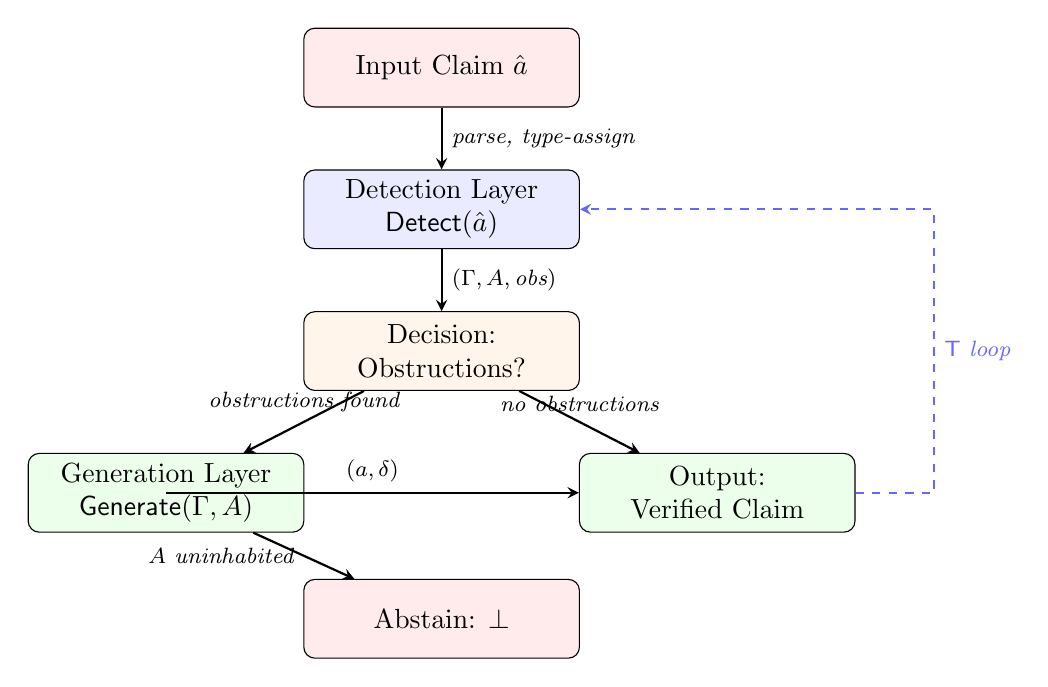
\begin{tikzpicture}[
  box/.style={draw, rounded corners, minimum width=3.5cm, minimum height=1cm, align=center, fill=blue!5},
  arrow/.style={->, thick, >=stealth},
  label/.style={font=\footnotesize\itshape}
]
% Main boxes
\node[box, fill=red!8] (input) at (0,6) {Input Claim $\hat{a}$};
\node[box, fill=blue!8] (detect) at (0,4.2) {Detection Layer\\$\Detect(\hat{a})$};
\node[box, fill=orange!8] (decide) at (0,2.4) {Decision:\\Obstructions?};
\node[box, fill=green!8] (generate) at (-3.5,0.6) {Generation Layer\\$\Generate(\Gamma, A)$};
\node[box, fill=green!8] (output) at (3.5,0.6) {Output:\\Verified Claim};
\node[box, fill=red!8] (abstain) at (0,-1) {Abstain: $\bot$};

% Arrows
\draw[arrow] (input) -- (detect) node[midway, right, label] {parse, type-assign};
\draw[arrow] (detect) -- (decide) node[midway, right, label] {$(\Gamma, A, \text{obs})$};
\draw[arrow] (decide) -- (generate) node[midway, above, label] {obstructions found};
\draw[arrow] (decide) -- (output) node[midway, above, label] {no obstructions};
\draw[arrow] (generate) -- (abstain) node[midway, left, label] {$A$ uninhabited};
\draw[arrow] (generate) |- (output) node[near end, above, label] {$(a, \delta)$};

% Feedback loop
\draw[arrow, dashed, blue!60] (output.east) -- ++(1,0) |- (detect.east) node[near start, right, label] {$\SemanticT$ loop};
\end{tikzpicture}
\caption{The HoTT-LM architecture implementing the semantic monad $\SemanticT = \Detect \circ \Generate$. The dashed blue arrow indicates the monadic feedback loop.}\label{fig:architecture}
\end{figure}

\subsection{The Generate-Check-Abstain Loop}

\begin{construction}[GCA Loop]\label{con:gca}
The Generate-Check-Abstain (GCA) loop implements the semantic monad as a practical algorithm:
\begin{enumerate}[nosep]
  \item \textbf{Generate}: The LLM produces a candidate claim $\hat{a}$.
  \item \textbf{Check}: The detection layer computes $\Detect(\hat{a}) = (\Gamma, A, \{o_1, \ldots, o_k\})$.
  \item \textbf{Decide}:
    \begin{itemize}[nosep]
      \item If $k = 0$ (no obstructions): output $\hat{a}$ as verified.
      \item If $k > 0$ and $A$ is inhabited: re-generate from $(\Gamma, A)$ to produce a corrected $(a, \delta)$.
      \item If $A$ is uninhabited: abstain ($\bot$).
    \end{itemize}
  \item \textbf{Iterate}: Apply the $\SemanticT$ monad up to $N$ times until convergence ($\SemanticT(\hat{a}) \cong \hat{a}$) or abstention.
\end{enumerate}
\end{construction}

\subsection{Persistent Homology for Real-Time Monitoring}

\begin{construction}[Topological Monitor]\label{con:topo-monitor}
During text generation, maintain a running Vietoris--Rips filtration on the embeddings:
\begin{enumerate}[nosep]
  \item Let $\{v_t\}_{t=1}^T$ be the sequence of embedding vectors during generation.
  \item At each step $t$, compute $\VR_\varepsilon(\{v_1, \ldots, v_t\} \cup S_{\mathcal{K}})$ where $S_{\mathcal{K}}$ is the knowledge base embedding set.
  \item Compute persistent homology across scales $\varepsilon \in [\varepsilon_{\min}, \varepsilon_{\max}]$.
  \item Flag hallucination if a persistent class $[\sigma] \in H_n$ with persistence $> \theta$ appears and the generation trajectory crosses its support.
\end{enumerate}
\end{construction}

\subsection{Architecture Diagram}

\begin{figure}[H]
\centering
\begin{tikzcd}[column sep=huge, row sep=huge]
\text{LLM} \arrow[r, "\text{generate}"] \arrow[d, "\text{embed}"'] & \mathsf{Claim} \arrow[r, "\Detect"] \arrow[d, "\text{parse}"] & \Sem \arrow[d, "\text{type-check}"] \\
\Vect \arrow[r, "\VR_\varepsilon"'] & \mathcal{K}_\bullet \arrow[r, "H_n"'] & \{[\sigma]\} \arrow[u, bend right, "\text{obstruction}"']
\end{tikzcd}
\caption{Data flow in the HoTT-LM POC. The upper path is the type-theoretic pipeline; the lower path is the topological pipeline. Both converge on obstruction detection.}\label{fig:dataflow}
\end{figure}


% ============================================================================
% 9. HASKELL FORMALIZATION
% ============================================================================
\section{Haskell Formalization}\label{sec:haskell}

We provide a standalone Haskell module implementing the key constructs of the synthesis framework. The complete code is available in the companion file \texttt{HoTTSynthesis.hs}.

\subsection{Core Types}

The semantic type system is formalized using GADTs:

\begin{lstlisting}[caption={Semantic types and terms}]
data SemType where
  Entity   :: String -> SemType
  Prop     :: String -> SemType
  DepType  :: SemType -> (SemTerm -> SemType) -> SemType
  PathType :: SemType -> SemTerm -> SemTerm -> SemType
  ProdType :: SemType -> SemType -> SemType
  SumType  :: SemType -> SemType -> SemType
  VoidType :: SemType
  UnitType :: SemType

data SemTerm where
  Grounded     :: String -> Source -> SemTerm
  Inferred     :: SemTerm -> Justification -> SemTerm
  PathWitness  :: SemTerm -> SemTerm -> PathEvidence -> SemTerm
  Refl         :: SemTerm -> SemTerm
  Hallucinated :: String -> SemTerm
\end{lstlisting}

\subsection{The Semantic Monad}

The semantic monad $\SemanticT = \Detect \circ \Generate$ is implemented as a Haskell monad:

\begin{lstlisting}[caption={The Semantic Monad}]
data SemanticM a = SemanticM
  { runSemantic :: Context -> KnowledgeComplex
                -> (a, [TopologicalObstruction]) }

instance Functor SemanticM where
  fmap f (SemanticM g) = SemanticM $ \ctx kc ->
    let (a, obs) = g ctx kc in (f a, obs)

instance Applicative SemanticM where
  pure a = SemanticM $ \_ _ -> (a, [])
  (SemanticM f) <*> (SemanticM x) = SemanticM $ \ctx kc ->
    let (fn, o1) = f ctx kc
        (a,  o2) = x ctx kc
    in (fn a, o1 ++ o2)

instance Monad SemanticM where
  (SemanticM m) >>= f = SemanticM $ \ctx kc ->
    let (a, o1)  = m ctx kc
        (b, o2)  = runSemantic (f a) ctx kc
    in (b, o1 ++ o2)
\end{lstlisting}

\subsection{Detection and Generation}

\begin{lstlisting}[caption={Detection and generation functions}]
detect :: SemTerm -> SemanticM DetectionResult
detect term = SemanticM $ \ctx kc ->
  let obstructions = findObstructions ctx kc term
      grounding    = checkGrounding ctx term
  in (DetectionResult grounding obstructions, obstructions)

generate :: SemType -> SemanticM (Maybe (SemTerm, Derivation))
generate goalType = SemanticM $ \ctx kc ->
  case searchInhabitant ctx kc goalType of
    Just (term, deriv) ->
      case typeCheck ctx term goalType of
        Right True -> ((Just (term, deriv)), [])
        _          -> (Nothing, [])
    Nothing -> (Nothing, [])
\end{lstlisting}

\subsection{The GCA Loop}

\begin{lstlisting}[caption={Generate-Check-Abstain loop}]
gcaLoop :: SemTerm -> SemType -> Int -> SemanticM GCAResult
gcaLoop claim goalType maxIter = go claim maxIter
  where
    go current 0 = return (GCAAbstain "max iterations")
    go current n = do
      result <- detect current
      case detectionObstructions result of
        [] -> return (GCAVerified current)
        obs -> do
          gen <- generate goalType
          case gen of
            Just (newTerm, deriv) -> go newTerm (n - 1)
            Nothing -> return (GCAAbstain "uninhabited type")
\end{lstlisting}

\subsection{All Five Obstruction Detectors}

\begin{lstlisting}[caption={Integrated obstruction detection}]
findObstructions :: Context -> KnowledgeComplex
                 -> SemTerm -> [TopologicalObstruction]
findObstructions ctx kc term = concat
  [ detectDisconnection ctx term        -- pi_0
  , detectCircularReasoning ctx term    -- pi_1
  , detectIncoherentPaths ctx term      -- pi_2
  , detectHomologicalHoles kc term      -- H_n
  , detectTransportAnomaly ctx term     -- holonomy
  ]
\end{lstlisting}


% ============================================================================
% 10. EXPERIMENTAL DESIGN
% ============================================================================
\section{Experimental Design}\label{sec:experiments}

We outline a rigorous experimental framework for validating the theoretical predictions.

\subsection{Experiment 1: Topological Detection Accuracy}

\begin{construction}[Synthetic Hallucination Benchmark]\label{con:benchmark}
Construct a benchmark with known hallucination types:
\begin{enumerate}[nosep]
  \item \textbf{Circular reasoning ($\pi_1$)}: Generate reasoning chains where the conclusion is used as a premise. Measure $\pi_1$ detection rate.
  \item \textbf{Unjustified inference ($\pi_0$)}: Generate claims connecting unrelated entities. Measure $\pi_0$ disconnection detection.
  \item \textbf{Inconsistent justifications ($\pi_2$)}: Generate claims with two contradictory but individually valid justifications. Measure $\pi_2$ detection.
  \item \textbf{Fabricated chains ($H_n$)}: Generate plausible but fabricated multi-step reasoning. Measure homological detection.
  \item \textbf{Compositional drift (holonomy)}: Generate text where meaning silently shifts through context changes. Measure holonomy detection.
\end{enumerate}
\end{construction}

\paragraph{Metrics.} For each hallucination type:
\begin{itemize}[nosep]
  \item \textbf{Precision}: fraction of detected hallucinations that are genuine (soundness measure).
  \item \textbf{Recall}: fraction of genuine hallucinations that are detected (completeness measure).
  \item \textbf{Topological specificity}: does the correct topological invariant activate for each type?
\end{itemize}

\subsection{Experiment 2: GCA Loop Efficacy}

\begin{construction}[GCA Evaluation]\label{con:gca-eval}
Evaluate the Generate-Check-Abstain loop:
\begin{enumerate}[nosep]
  \item Run a base LLM on questions with known answers.
  \item Wrap with the GCA loop (varying $N = 1, 2, 3$ iterations).
  \item Measure: hallucination rate reduction, abstention rate, answer quality on non-abstained responses.
\end{enumerate}
\end{construction}

\paragraph{Expected outcomes.}
\begin{itemize}[nosep]
  \item Hallucination rate should decrease monotonically with GCA iterations.
  \item Abstention rate should increase (the system correctly refuses to answer when uncertain).
  \item Answer quality on non-abstained responses should be higher than the base LLM.
  \item The system should converge (fixed point of $\SemanticT$) within 2--3 iterations.
\end{itemize}

\subsection{Experiment 3: Persistent Homology Monitoring}

\begin{construction}[Real-Time Topological Monitor]\label{con:monitor-eval}
During long-form text generation:
\begin{enumerate}[nosep]
  \item Compute persistent homology on sliding windows of embeddings.
  \item Track $H_0$ (connected components), $H_1$ (loops), $H_2$ (voids) across generation.
  \item Correlate topological events (birth/death of persistent features) with human-annotated hallucination instances.
\end{enumerate}
\end{construction}

\subsection{Experiment 4: Monad Convergence}

\begin{construction}[Monad Fixed-Point Analysis]\label{con:monad-convergence}
Empirically verify \Cref{cor:fixed-points}:
\begin{enumerate}[nosep]
  \item For a corpus of claims, compute $\SemanticT(\hat{a})$, $\SemanticT^2(\hat{a})$, $\SemanticT^3(\hat{a})$.
  \item Measure the distance $d(\SemanticT^k(\hat{a}), \SemanticT^{k+1}(\hat{a}))$ for increasing $k$.
  \item Verify that non-hallucinated claims are fixed points ($d \approx 0$ at $k = 1$) and hallucinated claims either converge to a corrected version or diverge to abstention.
\end{enumerate}
\end{construction}


% ============================================================================
% 11. DISCUSSION
% ============================================================================
\section{Discussion}\label{sec:discussion}

\subsection{The Nature of the Synthesis}

The central insight of this paper is that hallucination detection and correct generation are not independent problems requiring separate solutions, but \emph{dual} aspects of a single mathematical structure. The adjunction $\Generate \dashv \Detect$ is not merely a formal observation but encodes a deep principle: the ``best'' way to detect hallucination \emph{is} to attempt to regenerate the claim with full type-theoretic structure, and the ``best'' way to generate correctly \emph{is} to detect and avoid the topological obstructions that characterize hallucination.

The semantic monad $\SemanticT = \Detect \circ \Generate$ formalizes the ``generate-check'' loop that practitioners use informally (e.g., self-consistency decoding, chain-of-verification). Our contribution is to show that this loop has precise categorical structure---it is a monad---and that its fixed points are exactly the non-hallucinated claims (\Cref{cor:fixed-points}).

\subsection{Cubical Type Theory and Computational Content}

The HoTT framework gains computational content through cubical type theory \cite{cohen2018cubical}. In cubical type theory:
\begin{itemize}[nosep]
  \item Path types $a =_A b$ are represented as functions $I \to A$ from the interval $I$, with $p(0) = a$ and $p(1) = b$.
  \item The univalence axiom is provable (not postulated).
  \item Higher inductive types have computational rules.
\end{itemize}

For the semantic framework, cubical type theory provides:
\begin{itemize}[nosep]
  \item Constructive justification paths: a path $p\colon a =_A b$ is a \emph{concrete function} from $I$ to $A$, not merely an existence claim.
  \item Decidable type-checking: cubical type-checking is decidable \cite{angiuli2018cartesian}, making the $\Detect$ functor computable.
  \item Transport with computation: $\transport_p(x)$ reduces to a concrete term, enabling the $\Generate$ functor to produce explicit witnesses.
\end{itemize}

\subsection{Presheaf Models and Kripke--Joyal Semantics}

The $\infty$-topos $\mathcal{S}\mathrm{em}_\infty$ can be modeled concretely as a category of presheaves. Let $\mathcal{C}$ be the category of contexts (with morphisms being context extensions). Then:
\[
\mathcal{S}\mathrm{em}_\infty \simeq \PSh(\mathcal{C}) = [\mathcal{C}^{\op}, \Grpd]
\]
In this model:
\begin{itemize}[nosep]
  \item A semantic type $A$ is a functor $\mathcal{C}^{\op} \to \Grpd$ assigning to each context $\Gamma$ the $\infty$-groupoid $A(\Gamma)$ of valid claims of type $A$ in context $\Gamma$.
  \item A morphism $f\colon \Gamma \to \Delta$ induces restriction $f^*\colon A(\Delta) \to A(\Gamma)$.
  \item The internal logic is interpreted via Kripke--Joyal semantics: ``$A$ is true at $\Gamma$'' means $A(\Gamma)$ is inhabited.
\end{itemize}

This presheaf interpretation connects directly to the context-dependence of meaning and provides a model-theoretic foundation for the framework.

\subsection{Practical Considerations}

\paragraph{Computational complexity.} Full type inhabitation search is undecidable in general. For practical deployment, we restrict to:
\begin{itemize}[nosep]
  \item Bounded search depth for derivations.
  \item Approximate homology computation via persistent homology on embedding filtrations.
  \item Heuristic type assignment using the LLM itself as a ``type inference oracle.''
\end{itemize}

\paragraph{Hybrid architecture.} The POC architecture (\Cref{sec:architecture}) is designed as a \emph{wrapper} around existing LLMs, not a replacement. The LLM handles the ``creative'' generation; the type-theoretic layer handles verification. This parallels the proof-assistant paradigm where automation proposes proof steps and the kernel verifies them.

\paragraph{Scalability.} Persistent homology computation is $O(n^3)$ in the number of simplices (using standard persistence algorithms). For real-time monitoring during generation, we use:
\begin{itemize}[nosep]
  \item Sliding windows of bounded size.
  \item Incremental persistent homology updates \cite{dey2014computing}.
  \item Approximate algorithms for high-dimensional data.
\end{itemize}

\subsection{Limitations}

\begin{enumerate}[leftmargin=*]
  \item \textbf{Type assignment is hard.} Mapping natural language claims to formal semantic types is itself an open problem. Our framework assumes this mapping exists but does not solve it.
  \item \textbf{Knowledge base completeness.} The knowledge complex $\mathcal{K}_\bullet$ must be sufficiently rich to detect hallucinations. If the knowledge base itself has gaps, false negatives can occur.
  \item \textbf{Computational intractability.} Full HoTT type-checking in higher dimensions is computationally expensive. Practical implementations will require approximations.
  \item \textbf{The creative generation problem.} Type inhabitation search produces \emph{correct} but potentially \emph{boring} text. Balancing semantic correctness with creative generation is an open challenge.
\end{enumerate}

\subsection{Open Problems}

\begin{enumerate}[leftmargin=*]
  \item \textbf{Efficient type inhabitation for natural language.} Can the search be guided by the LLM's probability distribution while maintaining type-theoretic guarantees?
  \item \textbf{Incremental knowledge complex maintenance.} How should $\mathcal{K}_\bullet$ evolve as new knowledge arrives, and how does this affect existing homological features?
  \item \textbf{Higher-dimensional hallucination.} Are there hallucination types corresponding to $\pi_n$ for $n \geq 3$, and do they arise in practice?
  \item \textbf{Quantitative sheaf cohomology.} Can sheaf cohomology computations be made efficient enough for real-time detection?
  \item \textbf{The abstention--coverage tradeoff.} How to minimize abstention while maintaining zero hallucination rate?
\end{enumerate}


% ============================================================================
% 12. CONCLUSION
% ============================================================================
\section{Conclusion and Future Work}\label{sec:conclusion}

We have presented a unified framework for semantic correctness in language models that synthesizes topological hallucination detection and type-theoretic generation into a single coherent mathematical structure. The key results are:

\begin{enumerate}[leftmargin=*]
  \item The \textbf{Detection-Generation Duality}: detection and generation form an adjoint pair $\Generate \dashv \Detect$, revealing them as two sides of the same categorical coin.

  \item The \textbf{Semantic Monad}: the composite $\SemanticT = \Detect \circ \Generate$ is a monad whose fixed points are precisely the non-hallucinated claims.

  \item The \textbf{$\infty$-Topos Framework}: the ambient universe $\mathcal{S}\mathrm{em}_\infty$ is an $\infty$-topos with HoTT as its internal logic, providing a foundation in which both detection (type-checking) and generation (proof search) are native operations.

  \item The \textbf{Completeness Theorem}: the HHC together with type-theoretic generation gives a complete system---every hallucination is detected, and generation never produces undetected hallucinations.

  \item The \textbf{POC Architecture}: a concrete system wrapping LLMs with a type-checking layer, implementing the Generate-Check-Abstain loop with persistent homology monitoring.
\end{enumerate}

\paragraph{Future Work.} The immediate next steps are:
\begin{itemize}[nosep]
  \item Implementation of the POC in a production system, beginning with the persistent homology monitor.
  \item Development of efficient type assignment algorithms (natural language to HoTT types).
  \item Empirical validation on the experimental framework of \Cref{sec:experiments}.
  \item Extension to cubical type theory for constructive content.
  \item Investigation of the $\infty$-topos structure for multi-modal semantic types (text + image + audio).
\end{itemize}

The central message of this work is that hallucination is not a problem to be patched but a \emph{structural feature} of architectures that collapse the higher categorical structure of meaning. The solution is not better statistics but better mathematics: replacing the contractible codomain $\Vect$ with the richly-structured $\infty$-topos $\mathcal{S}\mathrm{em}_\infty$, and replacing probabilistic generation with certified type inhabitation. The adjunction $\Generate \dashv \Detect$ and the semantic monad $\SemanticT$ provide the organizing principle for this replacement.


% ============================================================================
% REFERENCES
% ============================================================================
\begin{thebibliography}{99}

\bibitem{angiuli2018cartesian}
C.~Angiuli, G.~Brunerie, T.~Coquand, R.~Harper, K.-B.~Hou, and D.~R.~Licata.
\newblock Cartesian cubical computational type theory: Constructive reasoning with paths and equalities.
\newblock In \emph{Proceedings of CSL 2018}, 2018.

\bibitem{bolt2019interacting}
J.~Bolt, B.~Coecke, F.~Genovese, M.~Lewis, D.~Marsden, and R.~Piedeleu.
\newblock Interacting conceptual spaces I: Grammatical composition of concepts.
\newblock In \emph{Proceedings of QPL 2019}, pages 151--181, 2019.

\bibitem{carlsson2009topology}
G.~Carlsson.
\newblock Topology and data.
\newblock \emph{Bulletin of the American Mathematical Society}, 46(2):255--308, 2009.

\bibitem{coecke2010mathematical}
B.~Coecke, M.~Sadrzadeh, and S.~Clark.
\newblock Mathematical foundations for a compositional distributional model of meaning.
\newblock \emph{Linguistic Analysis}, 36:345--384, 2010.

\bibitem{cohen2018cubical}
C.~Cohen, T.~Coquand, S.~Huber, and A.~M\"ortberg.
\newblock Cubical type theory: A constructive interpretation of the univalence axiom.
\newblock In \emph{Proceedings of TYPES 2015}, volume~69, pages 5:1--5:34, 2018.

\bibitem{curry2014sheaves}
J.~Curry.
\newblock Sheaves, cosheaves and applications.
\newblock \emph{arXiv preprint arXiv:1303.3255v2}, 2014.

\bibitem{dey2014computing}
T.~K.~Dey and Y.~Wang.
\newblock Computational topology for data analysis.
\newblock Cambridge University Press, 2022.

\bibitem{edelsbrunner2010computational}
H.~Edelsbrunner and J.~L.~Harer.
\newblock \emph{Computational Topology: An Introduction}.
\newblock American Mathematical Society, 2010.

\bibitem{hottbook}
The Univalent Foundations Program.
\newblock \emph{Homotopy Type Theory: Univalent Foundations of Mathematics}.
\newblock Institute for Advanced Study, 2013.

\bibitem{huang2023survey}
L.~Huang, W.~Yu, W.~Ma, W.~Zhong, Z.~Feng, H.~Wang, Q.~Chen, W.~Peng, X.~Feng, B.~Qin, and T.~Liu.
\newblock A survey on hallucination in large language models: Principles, taxonomy, challenges, and open questions.
\newblock \emph{arXiv preprint arXiv:2311.05232}, 2023.

\bibitem{ji2023survey}
Z.~Ji, N.~Lee, R.~Frieske, T.~Yu, D.~Su, Y.~Xu, E.~Ishii, Y.~J.~Bang, A.~Madotto, and P.~Fung.
\newblock Survey of hallucination in natural language generation.
\newblock \emph{ACM Computing Surveys}, 55(12):1--38, 2023.

\bibitem{johnstone2002sketches}
P.~T.~Johnstone.
\newblock \emph{Sketches of an Elephant: A Topos Theory Compendium}, volumes 1--2.
\newblock Oxford University Press, 2002.

\bibitem{lewis2020retrieval}
P.~Lewis, E.~Perez, A.~Piktus, F.~Petroni, V.~Karpukhin, N.~Goyal, H.~K\"uttler, M.~Lewis, W.-t.~Yih, T.~Rockt\"aschel, S.~Riedel, and D.~Kiela.
\newblock Retrieval-augmented generation for knowledge-intensive NLP tasks.
\newblock In \emph{NeurIPS 2020}, 2020.

\bibitem{li2025}
K.~Li et al.
\newblock Inference-time intervention: Eliciting truthful answers from a language model.
\newblock In \emph{NeurIPS 2023}, 2023.

\bibitem{long2026hhc}
M.~Long.
\newblock The Hallucination--Homotopy Correspondence: A complete classification of language model failure modes via algebraic topology and homotopy type theory.
\newblock \emph{GrokRxiv:2026.04.hallucination-homotopy-correspondence}, 2026.

\bibitem{long2026homotopical}
M.~Long.
\newblock Homotopical semantics for language models: Algebraic topological and homotopy type-theoretic approaches to the hallucination problem.
\newblock \emph{GrokRxiv:2026.04.yoneda-homotopical-semantics}, 2026.

\bibitem{lurie2009higher}
J.~Lurie.
\newblock \emph{Higher Topos Theory}.
\newblock Princeton University Press, 2009.

\bibitem{maclane1994sheaves}
S.~Mac~Lane and I.~Moerdijk.
\newblock \emph{Sheaves in Geometry and Logic: A First Introduction to Topos Theory}.
\newblock Springer-Verlag, 1994.

\bibitem{naitzat2020topology}
G.~Naitzat, A.~Zhitnikov, and L.-H.~Lim.
\newblock Topology of deep neural networks.
\newblock \emph{Journal of Machine Learning Research}, 21(184):1--40, 2020.

\bibitem{openai2023gpt4}
OpenAI.
\newblock GPT-4 technical report.
\newblock \emph{arXiv preprint arXiv:2303.08774}, 2023.

\bibitem{ouyang2022training}
L.~Ouyang et al.
\newblock Training language models to follow instructions with human feedback.
\newblock In \emph{NeurIPS 2022}, 2022.

\bibitem{robinson2014topological}
M.~Robinson.
\newblock \emph{Topological Signal Processing}.
\newblock Springer, 2014.

\bibitem{shulman2019all}
M.~Shulman.
\newblock All $(\infty,1)$-toposes have strict univalent universes.
\newblock \emph{arXiv preprint arXiv:1904.07004}, 2019.

\bibitem{voevodsky2010univalent}
V.~Voevodsky.
\newblock Univalent foundations.
\newblock Lecture at IAS, Princeton, 2010.

\end{thebibliography}


% ============================================================================
% APPENDIX A: CATEGORICAL DIAGRAMS
% ============================================================================
\appendix
\section{Key Commutative Diagrams}\label{app:diagrams}

\subsection{The Adjunction}

\begin{center}
\begin{tikzcd}[column sep=huge, row sep=huge]
\Sem \arrow[r, bend left=30, "\Generate"{name=F, above}] \arrow[dr, "\id"'] &
\mathsf{Claim} \arrow[l, bend left=30, "\Detect"{name=U, below}] \arrow[d, "\varepsilon"] \\
& \Sem \arrow[u, "\eta"']
\end{tikzcd}
\end{center}

\subsection{The Semantic Monad}

\begin{center}
\begin{tikzcd}[column sep=large, row sep=large]
\SemanticT^2 \arrow[r, "\mu"] \arrow[d, "\SemanticT\mu"'] & \SemanticT \arrow[d, equal] \\
\SemanticT^2 \arrow[r, "\mu"'] & \SemanticT
\end{tikzcd}
\qquad
\begin{tikzcd}[column sep=large, row sep=large]
\id \arrow[r, "\eta"] \arrow[dr, equal] & \SemanticT \arrow[d, "\mu"] & \id \arrow[l, "\SemanticT\eta"'] \arrow[dl, equal] \\
& \SemanticT
\end{tikzcd}
\end{center}

\subsection{The Functorial Collapse}

\begin{center}
\begin{tikzcd}[column sep=huge, row sep=large]
\Sem \arrow[r, "F"] \arrow[d, "\pi_n"'] & \Vect \arrow[d, "\pi_n"] \\
\pi_n(\Sem) \neq 0 \arrow[r, "F_*"'] & \pi_n(\Vect) = 0
\end{tikzcd}
\end{center}

\subsection{The Completeness Theorem}

\begin{center}
\begin{tikzcd}[column sep=large, row sep=large]
\hat{a} \arrow[r, "\Detect"] \arrow[d, "\varepsilon^{-1}"'] & (\Gamma, A, \text{obs}) \arrow[d, "\Generate"] \\
\Generate(\Detect(\hat{a})) \arrow[r, "\cong"'] & (a, \delta) \text{ or } \bot
\end{tikzcd}
\end{center}
The isomorphism $\varepsilon^{-1}$ exists if and only if $\hat{a}$ is not hallucinated (\Cref{thm:completeness}).

\subsection{The $\infty$-Topos Structure}

\begin{center}
\begin{tikzcd}[column sep=huge, row sep=large]
\mathcal{S}\mathrm{em}_\infty \arrow[r, hook, "\text{internal logic}"] & \text{HoTT} \\
\Grpd \arrow[u, "\text{objects}"] \arrow[r, "\text{nerve}"'] & \text{Simplicial Sets} \arrow[u, "\text{type theory}"']
\end{tikzcd}
\end{center}


% ============================================================================
% APPENDIX B: SUMMARY OF NOTATION
% ============================================================================
\section{Notation Summary}\label{app:notation}

\begin{center}
\begin{tabular}{lll}
\toprule
\textbf{Symbol} & \textbf{Meaning} & \textbf{Reference} \\
\midrule
$\Sem$ & Semantic category & \Cref{def:sem-cat} \\
$\mathsf{Claim}$ & Category of raw claims & \Cref{def:claim-cat} \\
$\Detect$ & Detection functor & \Cref{def:detect-functor} \\
$\Generate$ & Generation functor & \Cref{def:generate-functor} \\
$\SemanticT$ & Semantic monad $\Detect \circ \Generate$ & \Cref{def:semantic-monad} \\
$\mathcal{S}\mathrm{em}_\infty$ & $\infty$-topos of semantic types & \Cref{def:sem-topos} \\
$\mathcal{K}_\bullet$ & Simplicial knowledge complex & \Cref{def:knowledge-complex-review} \\
$\mathcal{F}$ & Semantic sheaf & \Cref{def:semantic-sheaf} \\
$H_n(\mathcal{K}_\bullet)$ & $n$-th homology group & \Cref{thm:hhc-review} \\
$H^n(\mathcal{K}_\bullet, \mathcal{F})$ & $n$-th sheaf cohomology & \Cref{thm:sheaf-obstruction} \\
$\pi_n$ & $n$-th homotopy group & \Cref{thm:hhc-classification-review} \\
$\Hall$ & Category of hallucination events & \cite{long2026hhc} \\
$\hTop$ & Category of pointed homotopy types & \cite{long2026hhc} \\
$\eta, \varepsilon$ & Unit and counit of adjunction & \Cref{thm:adjunction} \\
$\mu$ & Monad multiplication & \Cref{def:semantic-monad} \\
$a =_A b$ & Identity/path type & \Cref{def:semtype-review} \\
$A \simeq B$ & Semantic equivalence & \Cref{prop:univalence-filter} \\
\bottomrule
\end{tabular}
\end{center}


\end{document}
